\documentclass[12pt]{article}
\usepackage{times} 			% use Times New Roman font

\usepackage[margin=1in]{geometry}   % sets 1 inch margins on all sides
\usepackage{hyperref}               % for URL formatting
\usepackage[pdftex]{graphicx}       % So includegraphics will work
\setlength{\parskip}{1em}           % skip 1em between paragraphs
\usepackage{indentfirst}            % indent the first line of each paragraph
\usepackage{datetime}
\usepackage[small, bf]{caption}
\usepackage{listings}               % for code listings
\usepackage{xcolor}                 % for styling code
\usepackage{multirow}

%New colors defined below
\definecolor{backcolour}{RGB}{246, 246, 246}   % 0xF6, 0xF6, 0xF6
\definecolor{codegreen}{RGB}{16, 124, 2}       % 0x10, 0x7C, 0x02
\definecolor{codepurple}{RGB}{170, 0, 217}     % 0xAA, 0x00, 0xD9
\definecolor{codered}{RGB}{154, 0, 18}         % 0x9A, 0x00, 0x12

%Code listing style named "gcolabstyle" - matches Google Colab
\lstdefinestyle{gcolabstyle}{
  basicstyle=\ttfamily\small,
  backgroundcolor=\color{backcolour},   
  commentstyle=\itshape\color{codegreen},
  keywordstyle=\color{codepurple},
  stringstyle=\color{codered},
  numberstyle=\ttfamily\footnotesize\color{darkgray}, 
  breakatwhitespace=false,         
  breaklines=true,                 
  captionpos=b,                    
  keepspaces=true,                 
  numbers=left,                    
  numbersep=5pt,                  
  showspaces=false,                
  showstringspaces=false,
  showtabs=false,                  
  tabsize=2
}

\lstset{style=gcolabstyle}      %set gcolabstyle code listing

% to make long URIs break nicely
\makeatletter
\g@addto@macro{\UrlBreaks}{\UrlOrds}
\makeatother

% for fancy page headings
\usepackage{fancyhdr}
\setlength{\headheight}{13.6pt} % to remove fancyhdr warning
\pagestyle{fancy}
\fancyhf{}
\rhead{\small \thepage}
\lhead{\small HW\#3, TOMAR}  % EDIT THIS, REPLACE # with HW number
\chead{\small CS 532, Spring 2023} 

%-------------------------------------------------------------------------
\begin{document}

\begin{centering}
{\large\textbf{HW\#3 - Ranking Webpages}}\\ % EDIT THIS
                                % REPLACE # with HW num and ADD title
PRASHANT TOMAR\\                     % EDIT THIS
03/12/2023\\                      % EDIT THIS
\end{centering}

%-------------------------------------------------------------------------

% The * after \section just says to not number the sections
\section*{Q1}

\emph{ \textbf{Download the content of the 1000 unique URIs you gathered in HW2}}

\subsection*{Answer}
We will use the same file that contain 1000 unique links which was generated in HW 2 using IO operation, all the links will be retrieved and stored into the separate list. We will iterate over each link and perform below mention steps, 

\subsubsection*{1 - Retrieving the html-tags and html text  }

When the link is retrieve, it is encoded as ut-8 and then converted into hashed text. For this we have used \textit{hashlib} library.
\\ 
\begin{lstlisting}[language=Python, caption=Converting url to hash text]
import requests
import os
from bs4 import BeautifulSoup
import hashlib

def download_html(uri):
    response = requests.get(uri)
    if response.status_code == 200:
        return response.content
    else:
        return None

def generate_hash(uri):
    md5_hash = hashlib.md5(uri.encode())
    return md5_hash.hexdigest()

with open('clean.txt', 'r') as f:
    uri_list = f.readlines()

output_folder = 'output'
if not os.path.exists(output_folder):
    os.makedirs(output_folder)

batch_size = 10000

for batch_index in range(0, len(uri_list), batch_size):
    batch_uri_list = uri_list[batch_index:batch_index+batch_size]
    print("Processing URIs {}-{} out of {}: ".format(batch_index+1, batch_index+len(batch_uri_list), len(uri_list)))

    for index, uri in enumerate(batch_uri_list):
        uri = uri.strip()
        uri_hash = generate_hash(uri)
        print("Processing URI {}/{}: {}".format(index+1, len(batch_uri_list), uri))

        main_text_file = os.path.join(output_folder, 'main_text_{}.txt'.format(uri_hash))
        html_tags_file = os.path.join(output_folder, 'html_tags_{}.txt'.format(uri_hash))
        if os.path.exists(main_text_file) and os.path.exists(html_tags_file):
            print("Files already exist for URI: {}".format(uri))
            continue

        html_content = download_html(uri)
        if html_content is not None:
            soup = BeautifulSoup(html_content, 'html.parser')

            main_text = soup.get_text()

            with open(main_text_file, 'w', encoding='utf-8') as f:
                f.write(main_text)

            with open(html_tags_file, 'w', encoding='utf-8') as f:
                f.write(str(soup))

        else:
            print("Failed to download URI: {}".format(uri))
\end{lstlisting}

\subsubsection*{2 - Clean the name of the output files }

Next step we have written a separate function to change the file names of output folder corresponding to their hash values .
\\
\begin{lstlisting}[language=Python, caption=function to get response from each URI]
import os

folder_path = "main_text"

for filename in os.listdir(folder_path):
    
    if "main_text_" in filename:
        
        new_filename = filename.replace("main_text_", "")
        
        os.rename(os.path.join(folder_path, filename), os.path.join(folder_path, new_filename))
\end{lstlisting} 

\begin{lstlisting}[language=Python, caption=function to get response from each URI]
import os

folder_path = "html_tags"

for filename in os.listdir(folder_path):
    
    if "html_tags_" in filename:
        
        new_filename = filename.replace("html_tags_", "")
        
        os.rename(os.path.join(folder_path, filename), os.path.join(folder_path, new_filename))
\end{lstlisting} 

These file will be store in separate folders. As we have one more step to perform on these files.

\subsubsection*{3 - Clean the content of maintext files}

We will utilize the same content obtained from Step 2 and apply a cleaning process to it. To achieve this, we have developed a dedicated function that assists in cleaning the content. During this process, we will identify all the text files that include the stopword "coronavirus".
\\
\begin{lstlisting}[language=Python, caption=function to clean the html content]
import os
import shutil

root_folder = "main_text"

output_folder = "stopword_coronavirus"

keyword = "coronavirus"

def file_contains_keyword(file_path, keyword):
    with open(file_path, "r", encoding="utf-8") as f:
        content = f.read()
        if keyword in content:
            return True
    return False

for dirpath, dirnames, filenames in os.walk(root_folder):
    for filename in filenames:
        if filename.endswith(".txt"):
            file_path = os.path.join(dirpath, filename)
            if file_contains_keyword(file_path, keyword):
                output_file_path = os.path.join(output_folder, filename)
                shutil.move(file_path, output_file_path)
                print("Moved file:", filename)

\end{lstlisting} 

After parsing the content through this function, we will write the clean content into separate file with the file name using the same hashed text and store it into stopword "coronavirus" document.

\subsubsection*{4 - Save the hashed mapping of URIs}

Once the iteration is completed, we will save the hash mapping to separate csv file that will be used in question 3 to create ranking tables.
\\
\begin{lstlisting}[language=Python, caption=Hash mapping conversion to csv]
import hashlib

with open('clean.txt', 'r') as f:
    uri_list = f.readlines()

def generate_hash(uri):
    md5_hash = hashlib.md5(uri.encode())
    return md5_hash.hexdigest()

uri_hash_map = {}

for i, uri in enumerate(uri_list):
    uri_hash_map[uri.strip()] = (i+1, generate_hash(uri))

with open('uri_hash_map.csv', 'w') as f:
    f.write("serial_number,uri,hash_value\n")
    for uri, values in uri_hash_map.items():
        f.write(f"{values[0]},{uri},{values[1]}\n")


\end{lstlisting}
\clearpage

\section*{Q2}

\emph{ \textbf{Rank with TF-IDF}}

\subsection*{Answer}
\subsubsection*{1 - Choose the term and select 10 document from processed folder}

Our task is to go through the documents in the processed folder and search for the term 'coronavirus' in each one. Those that contain this term will be moved to a separate folder. We will select and copy 10 such documents to the new folder.

\begin{lstlisting}[language=Python, caption=Copy files that contain the term to separate folder]
import os
import numpy as np

from pandas import DataFrame

idf = np.round(np.log2(60000000000 / 3730000000), 3)

rows = []
count = 0
for item in os.listdir('stopword_coronavirus/'):
    if count == 10:
        break
    with open('stopword_coronavirus/' + item, 'r', encoding='utf-8') as filehandle:
        file_content = filehandle.read().lower()

    word_count = len(file_content.split())
    term_count = file_content.count('coronavirus')

    term_freq = np.round(term_count / word_count, 3)
    tf_idf = np.round(term_freq * idf, 3)

    rows.append([item, term_freq, idf, tf_idf])
    count += 1

result = DataFrame(rows, columns=['File', 'TF', 'IDF', 'TF-IDF'])
result.to_csv('rank-tf-idf.csv')
print(result)

\end{lstlisting}

\subsubsection*{2 - Calculate TF, IDF and TF-IDF for each link }

During this stage, our objective is to compute TF, IDF, and TF-IDF values for each document. To obtain TF scores, we will analyze each document and retrieve the number of occurrences of the term 'coronavirus' in addition to the total word count of the document.

We will employ the following formula to determine Term Frequency:

\begin{equation}\label{eq1}
Term\_Frequency = \frac{Term\_count\_in\_document}{Total\_word\_in\_document}
\end{equation}

We have lowered case all the content before searching the term to get the count accurate. Also we have count the total word by splitting up the text by space in content file which return the array of word and using \textit{len} python string function to count the length.

To calculate IDF, we will use google search to find the total count in corpus for the term \textit{coronavirus}. As we are using google the total document index will be 60B. Refer figure 1.

\begin{figure}[h]
\caption{Chart from worldwidewebsize.com}
\centering
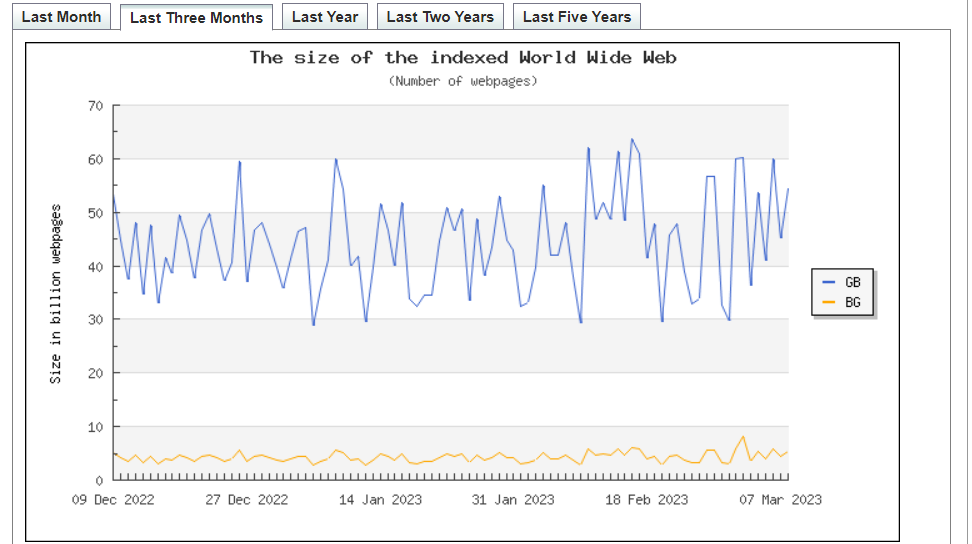
\includegraphics[width=0.70\textwidth]{wwwsize.png}
\end{figure}

Figure 2, represent the result of the term coronavirus in google.com. You can see that the size of the search term in corpus is \textit{3,730,000,000}

\begin{figure}[h]
\caption{Searching results for the term coronavirus in google.com}
\centering

\includegraphics[width=0.70\textwidth]{googlecorpus.png}
\end{figure}

We will use these values and calculate the IDF by the following equation, 

\begin{equation}\label{eq1}
IDF = \log_2({\frac{Total\_docs\_in\_corpus}{Total\_docs\_with\_terms}})
\end{equation}
\clearpage
Once the TF and IDF is calculated, we will use the following equation to calculate TFIDF,

\begin{equation}\label{eq1}
TF\_IDF = TF * IDF
\end{equation}
\\
\begin{lstlisting}[language=Python, caption=Complete implementation for calculating TF IDF and TFIDF]

import os
import numpy as np

from pandas import DataFrame

idf = np.round(np.log2(60000000000 / 3730000000), 3)

rows = []
count = 0
for item in os.listdir('stopword_coronavirus/'):
    if count == 10:
        break
    with open('stopword_coronavirus/' + item, 'r', encoding='utf-8') as filehandle:
        file_content = filehandle.read().lower()

    word_count = len(file_content.split())
    term_count = file_content.count('coronavirus')

    term_freq = np.round(term_count / word_count, 3)
    tf_idf = np.round(term_freq * idf, 3)

    rows.append([item, term_freq, idf, tf_idf])
    count += 1

result = DataFrame(rows, columns=['File', 'TF', 'IDF', 'TF-IDF'])
result.to_csv('rank-tf-idf.csv')
print(result)

\end{lstlisting}
\clearpage
Figure 3, shows the result ,
\begin{figure}[h]
\caption{Print result of the calculated table}
\centering
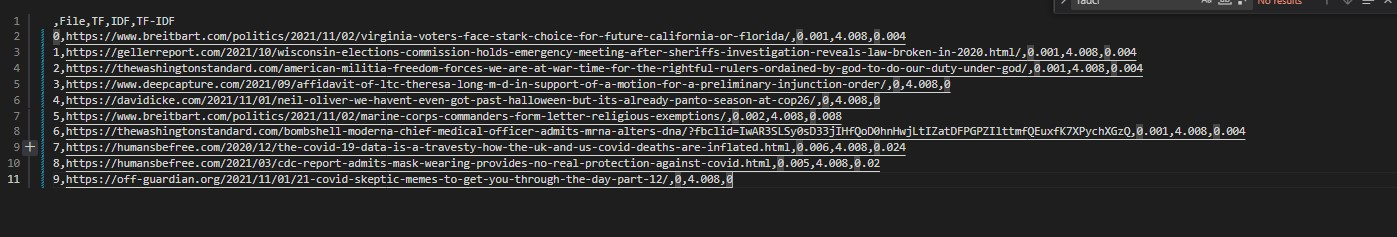
\includegraphics[width=\textwidth]{1.jpg}
\end{figure}

The result is shared in the table 1,

\begin{table}[h]
\centering
\caption{TF, IDF and TFIDF table}
\label{tbl:simple}
\begin{tabular}{p{0.50\linewidth}p{0.15\linewidth}p{0.15\linewidth}p{0.15\linewidth}}
\hline
\textbf{URIs} & \textbf{TF} & \textbf{IDF} & \textbf{TFIDF} \\ \hline \hline
\url{https://www.breitbart.com/} & 0.001 & 4.008 & 0.004 \\ \hline
\url{https://gellerreport.com/} & 0.001 & 4.008 & 0.004 \\ \hline
\url{https://thewashingtonstandard.com} & 0.001 & 4.008 & 0.004 \\ \hline
\url{https://www.deepcapture.com} & 0 & 4.008 & 0 \\ \hline
\url{https://davidicke.com} & 0 & 4.008 & 0 \\ \hline
\url{https://www.breitbart.com/politics} & 0.002 & 4.008 & 0 \\ \hline
\url{https://thewashingtonstandard.com} & 0.001 & 4.008 & 0.004 \\ \hline
\url{https://humansbefree.com/2020/12} & 0.006 & 4.008 & 0.024 \\ \hline
\url{https://humansbefree.com/2021/03/} & 0.005 & 4.008 & 0.002 \\ \hline
\url{https://off-guardian.org/} & 0 & 4.008 & 0 \\ \hline

\end{tabular}
\end{table}

\clearpage

\section*{Q3}

\emph{ \textbf{Now rank the domains of those 10 URIs from Q2 by their PageRank.}}

\subsection*{Answer}
For this we have used \url{https://www.checkpagerank.net/check-page-rank.php} to found the ranks of the processed web pages.

Result of the ranks have been shared in below table, 


\begin{table}[h]
\centering
\caption{Web pages ordered with respect to their ranks}
\label{tbl:simple}
\begin{tabular}{p{0.50\linewidth}p{0.20\linewidth}}
\hline
\textbf{URIs} & \textbf{Ranks}  \\ \hline \hline
\url{https://www.breitbart.com} & 0.8 \\ \hline \hline
\url{https://www.breitbart.com/politics} & 0.8 \\ \hline \hline
\url{https://davidicke.com} & 0.7 \\ \hline \hline
\url{https://off-guardian.org/} & 0.6 \\ \hline \hline
\url{https://gellerreport.com} & 0.5 \\ \hline \hline
\url{https://humansbefree.com/2020/12/}	 & 0.5 \\ \hline \hline
\url{https://humansbefree.com/2021/03} &	0.5 \\ \hline \hline
\url{https://www.deepcapture.com} & 0.5 \\ \hline \hline
\url{https://thewashingtonstandard.com} & 0.5  \\ \hline \hline
\url{https://thewashingtonstandard.com} & 0.5 \\ \hline \hline




\end{tabular}
\end{table}

After analyzing and comparing the ranking with the tables displaying TF, IDF, and TF-IDF results, we can conclude that the frequency of terms used in web pages with high rankings is generally low. This suggests that other factors, such as meta tags, site references, etc., have a significant impact on the ranking of web pages.
\clearpage

\section*{Q4}

\emph{ \textbf{Compute the Kendall Tau-b score}}

\subsection*{Answer}
Now we will calculate the Kendall Tau score for the lists from Q2 and Q3
\\

\begin{lstlisting}[language=Python, caption=Code for creating local corpus]
from scipy.stats import kendalltau

# Define the two lists
list1 = [1, 2, 3, 4, 5, 6, 7, 8, 9, 10]
list2 = [1, 5, 9, 8, 3, 2, 10, 6, 7, 4]

# Compute the Kendall Tau_b score and p-value
tau, p_value = kendalltau(list1, list2)

# Print the results to a file
with open("kendalltau_results.txt", "w") as f:
    print("Tau_b score: ", tau, file=f)
    print("p-value: ", p_value, file=f)
\end{lstlisting}

The Tau-b score is 0.1111111111111111 and p-value:  0.7274895282186948


\clearpage


\section*{Q5}

\emph{ \textbf{Build a simple (i.e., no positional information) inverted file (in ASCII) for all the words from your 1000 URIs}}

\subsection*{Answer}
We generated an inverted index file using the processed folder. To do this, we accessed the files from the processed folder, iterated through each file, and extracted the content. We then used the split function to break down the content by space, in order to retrieve all the words. After retrieving all the words, we cleaned the data by removing special characters from each word and stored them in a separate list.

As there must be a chance of word repetition, we used python data structure \textit{set} to make the list of word unique. After the final list is generated, we write the result to file.


\\

\begin{lstlisting}[language=Python, caption=Implementation for creating inverted index file]
import os
from shutil import copy
import numpy as np

inverted_index = []

for file_name in os.listdir('main_text/'):
    with open(os.path.join('main_text', file_name), 'r', encoding='utf-8') as f:
        content = f.read().lower()
        tokens = content.split()

        clean_tokens = [token.strip('''!()-[]{};:'"\, <>./?@#$%^&*_~–''') for token in tokens]

        unique_tokens = set(filter(None, clean_tokens))

        inverted_index.extend(list(unique_tokens))

unique_tokens = list(set(inverted_index))

with open('inverted_file.txt', 'w', encoding='utf-8') as f:
    f.write('\n'.join(unique_tokens) + '\n')


\end{lstlisting}

\clearpage


\section*{References}



\begin{itemize}
    \item {Hashlib library, \url{https://docs.python.org/3/library/hashlib.html}}
    \item {Page Rank, \url{http://www.prchecker.info/check_page_rank.php}}
    \item {Request Documentation, \url{https://requests.readthedocs.io/en/master/user/quickstart/#response-content}}
    \item {Boilerpy3 reference, \url{https://pypi.org/project/boilerpy3/	}}
    \item {Github, \url{https://github.com/odu-cs432-websci/spring23-hw3-Badjedi04}}

\end{itemize}

\end{document}


